\onecolumn
\part*{はじめに}
\addcontentsline{toc}{section}{はじめに}

本書はタイピング界の住人がタイピングについて好きなように好きなだけ文章を書いた、という世にも珍しいタイピング専門誌です。それだけに、同じようにタイピングに興味を持つ人にとっては身震いするほど面白い記事ばかりで構成されています。そうでない人は「え?タイピングってキーボード打つだけでしょ」というイメージを持っているかもしれませんが、普段何気なく打っているキーボード、そしてタイピングの奥深さを知る良いきっかけになるでしょう。「競技タイピングの入門」「競技タイピングに取り組む上での練習方法」「キーボード配列を変えることのすすめ」「タイピングの指使い」「伝説的タイパーやソフト作者のインタビュー」など多種多様な内容を取りそろえているので、興味のある方はこんなところは読み飛ばして目次から好きな記事へと飛んでください。\\

さて、「そうでない人」はそもそも「タイピング界」というこの耳慣れぬ言葉に戸惑う方も多いかも知れません。一言で言えばキーボードを使ったタイピングが好き、あるいは興味を持っている人たちで構成されているコミュニティのような大枠を表しています。ただ、SNSサービスにおけるコミュニティと異なるのは、タイピング界に属する全員が全員互いにコミュニケーションを取り合うような関係ではない、ということです。あるタイピングゲームを好きな人たちだけで盛り上がっているコミュニティや、キーボードに関する研究をしているコミュニティ、2chのような特定の場所でのみ交流を行っている人たちなど、興味の対象や交流の場について様々な形でタイピングに関わっている人たちをすべて包括しているのがタイピング界です。
これは、あるゲームジャンルを好きな人で構成されている「格ゲー界」や「シューティングゲーム界」といったものと同じです。ただ、ゲームとタイピングで大きく異なるのが、タイピングは純粋なるゲーム要素だけではないということです。現代では多くの人がPCに触れ、キーボードを使って文章を入力していると思います。多くのゲーマーにとってのゲームは「目的」であり、多くの人にとってのタイピングは「手段」であると思いますが、その中でタイピングを「目的」として活動している人たちで構成されるのがタイピング界なのです。特に競技タイピングに取り組んでいる人たちを「タイパー」と呼んでいます。

タイピングに興味のない人がタイパーを見かけると「この人はなぜキーボードを打ってて楽しそうなんだろう?」と思うかも知れませんし、勢い余って「キモい」と言ってしまうことがあるかも知れません\footnote{一部の人にとってはご褒美です}。そのように感じてしまうのも無理はありませんが、実際に「タイピング」という一定時間内に入力できる文字数を競う競技が存在する以上、これは短距離走や競輪のようなものと一緒なのです。多くの人にとって自転車に乗るときのフォームは関心の対象外で、さらに乗れるようになったあとに自転車に乗る練習をするなんてことはありません。ではなぜ、競輪選手はフォームを気にして練習するのか。それはより速く走り、競争に勝ち、栄誉を手にしたいからです。タイパーも同じで、誰よりも速く、正確なタイピングを身につけてライバルに勝つためにキーボードを\ruby{叩}{たた}いているのです。競輪選手になるには競輪学校に入り、普通のシティサイクルの数十倍もする自転車を買わなければなりませんが、タイパーになるにはどこにでも売っているPCとキーボードがあれば大丈夫です。そういう意味では大変敷居が低く\footnote{小学生のうちからトップレベルのタイパーとなった人もいます}、実用的なスポーツであると言えます。本書はタイパーの語る練習やタイピング観が盛りだくさんなので、そういう視点から読んでみるのも面白いかもしれません。\\

10年以上の歴史を持つタイピング界で培われてきた技術や知識、そして未だにタイピングが愛され続けている理由、多くの読者がその一端に触れられますように。

\begin{flushright}
2011年12月 タイピングガチ勢一同
\end{flushright}

\part*{本書が必要とするものについて}
タイピング界に対する寛容な心

\part*{本書の構成}
本書は全体を通して一本の筋道があるわけではなく、どこから読んでも構わないアラカルト形式です。大きく分けると、前半がタイピングに関する様々な観点からの文章で構成されており、後半がインタビュー集になっています。タイピング初心者が本書を手にとっているとは考えづらいですが、前半はやはりある程度タイピングに慣れている方を対象としています。後半のインタビュー集に関しては全力全開でタイピング界向けの記事になっています。インタビューにご協力いただいた方をご存知の読者にとってはここでしか読めない\ruby{垂涎}{すいぜん}ものの内容です。とは言いつつ、そうでない人にとっても実は興味深いものが多いです。昔からタイピング界に携わっている人たちのインタビューを読むことで、タイピング界がどのように形成されていったか、どのような人たちが関わってきたかを知る良いチャンスになるはずです。

\section*{Typin' Girls はじめての競技タイピング \small{by W/H}}
\noindent 対象読者:「タイパーとか競技タイピングって何?」\\
本書の中でも一風変わった小説スタイル。フィクションを通して面白おかしくタイピング界へと誘います。

\section*{タイピング練習論 \small{by テル(vuttar)}}
\noindent 対象読者:「すでにある程度練習を重ねているタイパー」\\
がむしゃらに打つだけでは成長しなくなってきた。そんなタイパーに向けたトップタイパーの練習方法です。

\section*{新配列のすすめ \small{by kouy}}
\noindent 対象読者:「今使っているローマ字入力やかな入力に不満がある」\\
キーボード配列を変えることで日本語をもっと楽に打つことができます。配列変更の入門記事。

\section*{高速化のための配列習得 \small{by tomoemon}}
\noindent 対象読者:「より速く打つためにキーボード配列を変えようと思っている」\\
キーボード配列がいろいろあることは知っているけど\ruby{躊躇}{ちゅうちょ}している、というタイパーに向ける経験談です。

\section*{「打ちやすい」キーボード配列を求めて \small{by nooyosh}}
\noindent 対象読者:「キーボード配列を設計してみたいと考えている」\\
キーボード配列設計に関する理論的な分析です。今回は設計までは至りませんが重要な考え方が満載です。

\section*{タイピングとキーボード \small{by eigh8\_t}}
\noindent 対象読者:「キーボード選びに迷っている」\\
タイピングといえば欠かせないのがキーボード。タイピングにどのような影響を与えているのでしょうか。

\section*{英語タイピング \small{by テル(vuttar)}}
\noindent 対象読者:「世界に飛び出したい」\\
日本語タイピングの競技者は日本人だけですが、英語タイピングは世界が相手です。さらなる戦場を求めるタイパーへ。

\section*{我流運指 underground \small{by o-ck}}
\noindent 対象読者:「自分のキーボードを打つ指使いに不安を覚えている」\\
ホームポジションとは一体何だったのか。彼らの指はキーボード上でいかなる制約も受けずに飛び回ります。

\section*{鍵盤打鍵者たちが考えること - Masterminds of Typing \small{by W/H}}
\noindent 対象読者:「本書の読者」\\
タイピング界に名を知らぬものはいないタイパー、タイピングソフトの作者をそろえた豪華インタビュー。

\part*{本書の表記}
\textbf{キーボード上のキー}\\
通常の文字と区別するため、キーボードのキーについては四角で囲んで表記しています。\\
例:\key{A}のキーを単独で押すと「a」、\keydouble{Shift}{A}のように\key{Shift}と合わせて押すと大文字の「A」になります。

\textbf{キーボードの指使い}\\
キーをどの指で打つか、本書では下図のようにそれぞれの指に番号をふり、\finger{12345}のように下線付きで表記します。
\noindent 例:「か」と入力するには\key{K}\key{A}を\finger{81}で打ちます。

\vspace{3mm}
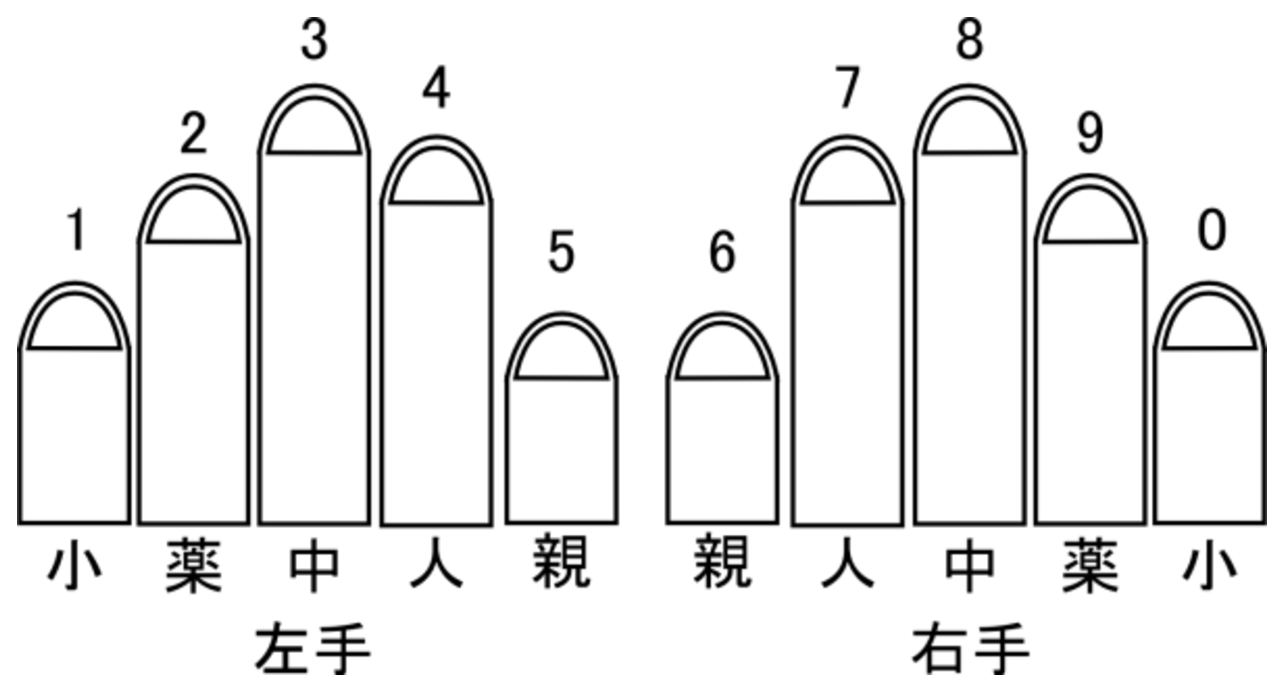
\includegraphics[width=13cm,clip]{res_tomoemon/finger.eps}
\vspace{-4mm}

\part*{意見と質問}
本書の執筆にあたってできる限りの確認をしていますが、誤字・脱字や誤解・混乱を招くような表現、内容が含まれている可能性があります。ささいなことでも構わないので気づいたことは執筆陣へご連絡いただけると幸いです。連絡は、本書の最後に載せている、執筆陣のtwitterやブログへお願いします。

\part*{謝辞}
本書の執筆にあたり、多忙なる中、快くインタビューにご協力してくださった、Pocariさん、dqmaniacさん、たにごんさん、むなしいさん、俺さん、Quvotaさん、父・信仁さん、あきうめさん、モルタルコさん、GANGASさん、えむさん、そして勃起教教祖さんに心より感謝いたします。特に、インタビューのセッティングからレビューの取りまとめに至るまで、窓口となって全面的にご協力頂いた Pocari さんには、格別の感謝の意を表します。執筆陣だけでは語ることのできない非常に密度の高い内容を盛り込むことができました。また、執筆陣の要望を聞いて表紙のイラストを描いてくださったcreamさん、サークル名を決める際にすかさず名前を挙げてくださったグミさんに感謝します。その他、執筆陣へのご助力や宣伝にご協力してくださったみなさん、ありがとうございます。最後に、これまでタイピングに取り組んで様々な経験と知識を残してくださったタイピング界に関わるすべてのみなさんのおかげで本書は完成しました。本当にありがとうございます。

